\documentclass[dvisvgm, border=5mm]{minimal}
\usepackage{tikz}

\usetikzlibrary{arrows.meta}

\special{background White}

\begin{document}

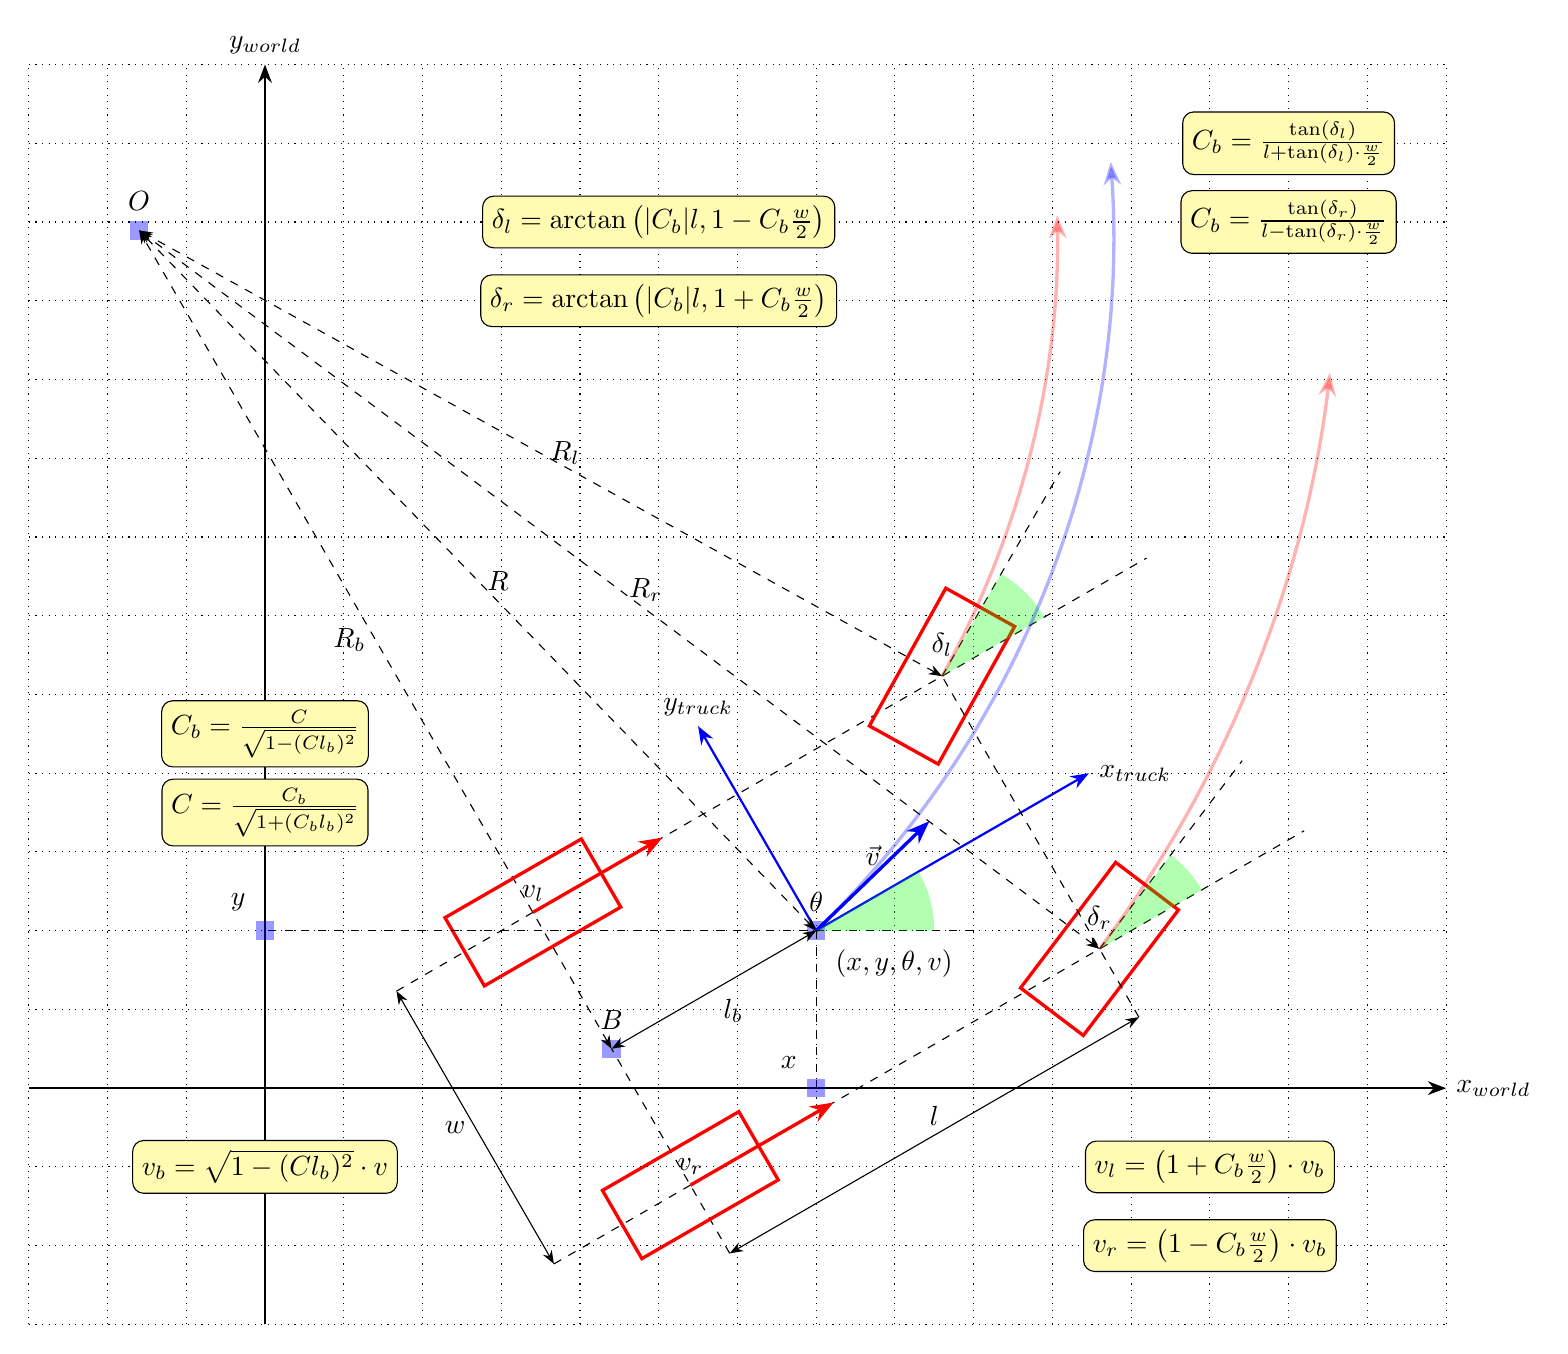
\begin{tikzpicture}[>=Stealth]
    % world axes
    \draw[step=1, dotted] (-3,-3) grid (15,13);
    \draw[->, thick] (-3,0) -- (15,0) node[right] {$x_{world}$};
    \draw[->, thick] (0,-3) -- (0,13) node[above] {$y_{world}$};

    \begin{scope}[shift={(7,2)}, rotate=30]
        % truck axes
        \draw[->, blue, thick] (0,0) -- (4,0) node[black, right] {$x_{truck}$};
        \draw[->, blue, thick] (0,0) -- (0,3) node[black, above] {$y_{truck}$};

        % base points
        \node[fill=blue, opacity=0.4, label=above:{$O$}] at (-3,12) {};
        \node[fill=blue, opacity=0.4, label={below right:{$(x,y,\theta,v)$}}] at (0,0) {};
        \node[fill=blue, opacity=0.4, label={above:{$B$}}] at (-3,0) {};

        % axial guides
        \draw[dashed] (-5,-2) -- (6,-2);
        \draw[dashed] (-5,2) -- (6,2);

        % steering guides
        \draw[<->, black, dashed] (-3, 0) -- (-3,12) node[left, midway] {$R_b$};
        \draw[black, dashed] (-3, -3) -- (-3,0);

        \draw[<->, black, dashed] (0,0) -- (-3,12) node[right, midway] {$R$};
        \draw[<->, black, dashed] (3,2) -- (-3,12) node[right, midway] {$R_l$};
        \draw[<->, black, dashed] (3,-2) -- (-3,12) node[right, midway] {$R_r$};

        % rear tyres
        \draw[red, very thick] (-4.0,+1.5) rectangle (-2.0,+2.5);
        \draw[red, very thick] (-4.0,-2.5) rectangle (-2.0,-1.5);

        % front tires
        \draw[red, very thick, shift={(3,2)}, rotate=30.96] (-1.0,-0.5) rectangle (+1.0,+0.5);
        \draw[red, very thick, shift={(3,-2)}, rotate=22.85] (-1.0,-0.5) rectangle (+1.0,+0.5);

        % front guides
        \draw[black, dashed] (3,-3) -- (3,2);
        \draw[black, dashed, shift={(3,2)}, rotate=30] (0,0) -- (3,0);
        \draw[black, dashed, shift={(3,-2)}, rotate=22.85] (0,0) -- (3,0);

        % width
        \draw[<->] (-5,-2) -- (-5,2) node[left, midway] {$w$};

        % from rear to base
        \draw[<->] (-3,0) -- (0,0) node[midway, below right] {$l_b$};

        % length
        \draw[<->] (-3,-3) -- (3,-3) node[midway, above] {$l$};

        % front angles
        \fill[green, opacity=0.3] (3,2) -- (4.5,2) arc [start angle=0, end angle=30, radius=1.5];
        \node[label=above:{$\delta_l$}] at (3,2) {};

        \fill[green, opacity=0.3] (3,-2) -- (4.5,-2) arc [start angle=0, end angle=22.85, radius=1.5];
        \node[label=above:{$\delta_r$}] at (3,-2) {};

        % path
        \draw[->, blue, very thick, opacity=0.3, rotate=14.04] (0,0) arc [start angle=-90, end angle=-40, radius=12.37];
        \draw[->, red, very thick, opacity=0.3, shift={(3,2)}, rotate=30.96] (0,0)  arc [start angle=-90, end angle=-60,radius=11.66];
        \draw[->, red, very thick, opacity=0.3, shift={(3,-2)}, rotate=23.20] (0,0)  arc [start angle=-90, end angle=-60,radius=15.23];

        % velocity
        \draw[->, blue, very thick, rotate=14.04] (0,0) -- (2,0) node[black, midway, above] {$\vec{v}$};
        \draw[->, red, very thick] (-3,2) node[black, above]{$v_l$} -- (-1.10,2);
        \draw[->, red, very thick] (-3,-2) node[black, above]{$v_r$} -- (-0.90,-2);
    \end{scope}

    % pose
    \draw[dashed] (7,2) -- (7,0) node[fill=blue, opacity=0.4, label=above left:{$x$}] {};
    \draw[dashed] (9,2) -- (0,2) node[fill=blue, opacity=0.4, label=above left:{$y$}] {};

    \fill[green, opacity=0.3] (7,2) -- (8.5,2) arc [start angle=0, end angle=30, radius=1.5];
    \node[label=above:{$\theta$}] at (7, 2) {};

    % hints
    \draw (12,-1) node[fill=yellow!30, draw, rounded corners] {$v_l = \big(1 + C_b \frac{w}{2} \big) \cdot v_b$};
    \draw (12,-2) node[fill=yellow!30, draw, rounded corners] {$v_r = \big(1 - C_b \frac{w}{2} \big) \cdot v_b$};

    \draw (5,11) node[fill=yellow!30, draw, rounded corners] {$\delta_l = \arctan \big(|C_b| l, 1 - C_b \frac{w}{2} \big)$};
    \draw (5,10) node[fill=yellow!30, draw, rounded corners] {$\delta_r = \arctan \big(|C_b| l, 1 + C_b \frac{w}{2} \big)$};


    \draw (0, 4.5) node[fill=yellow!30, draw, rounded corners] {$C_b = \frac{C}{\sqrt{1 - (C l_b)^2}}$};
    \draw (0, 3.5) node[fill=yellow!30, draw, rounded corners] {$C = \frac{C_b}{\sqrt{1 + (C_b l_b)^2}}$};

    \draw (0, -1) node[fill=yellow!30, draw, rounded corners] {$v_b = \sqrt{1 - (C l_b)^2} \cdot v$};

    \draw (13, 12) node[fill=yellow!30, draw, rounded corners] {$C_b = \frac{\tan(\delta_l)}{l + \tan(\delta_l) \cdot \frac{w}{2}}$};
    \draw (13, 11) node[fill=yellow!30, draw, rounded corners] {$C_b = \frac{\tan(\delta_r)}{l - \tan(\delta_r) \cdot \frac{w}{2}}$};

\end{tikzpicture}
\end{document}
